\documentclass{article}
\usepackage{mathrsfs} % for scripts
\usepackage{standalone}
\usepackage{tikz}
\usetikzlibrary{hobby}
\begin{document}
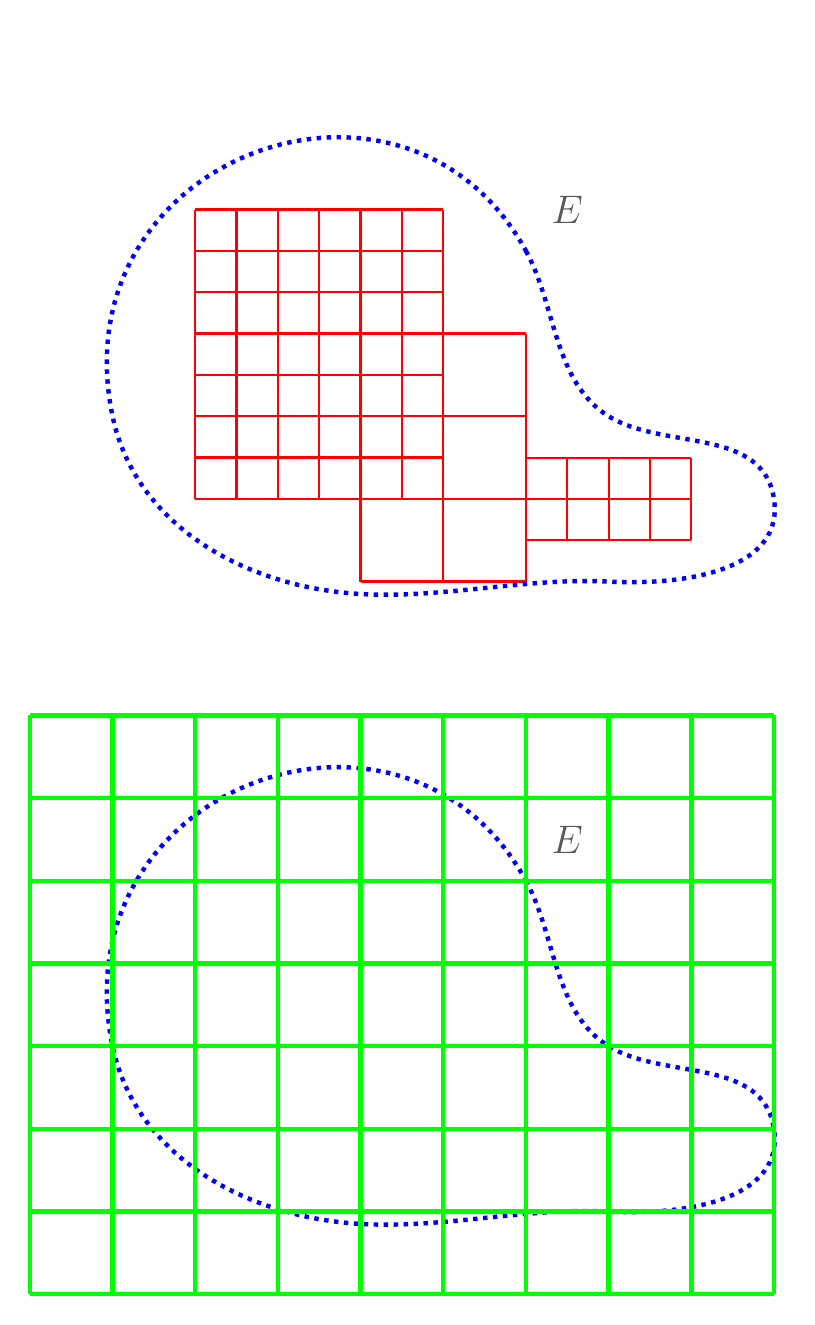
\begin{tikzpicture}
    \begin{scope}[scale=1.05,closed hobby,fill opacity=0.65]
	\node at (0.5,3.5) {\Large$E$};
	\draw[step=1.0cm,red,thick] (-2,-1) grid (0,2);
	\draw[step=1.0cm,red,thick] (-2,0) grid (-4,2);
	\draw[step=0.5cm,red,thick] (-4,0) grid (-1,3.5);
	\draw[step=0.5cm,red,thick] (0,-0.5) grid (2,0.50);
	%\draw[ultra thick,red] (-2.5,0) rectangle (-0.5,2);
	\draw[ultra thick,dotted,blue] plot coordinates {( 0,3)(1,1)(3,0)(1,-1)(-2,-1.15)(-5.0,1)} ;
    \end{scope}
    \begin{scope}[yshift=-8cm,scale=1.05,closed hobby,fill opacity=0.65]
	\node at (0.5,3.5) {\Large$E$};
	\draw[ultra thick,dotted,blue] plot coordinates {( 0,3)(1,1)(3,0)(1,-1)(-2,-1.15)(-5.0,1)} ;
	\draw[step=1.0cm,green,ultra thick](3,-2) grid (-6,5);
    \end{scope}
	\end{tikzpicture}
\end{document}
